\documentclass[aspectratio=169]{beamer}
\usepackage[utf8]{inputenc}
\usepackage{hyperref}
\usepackage{amsmath,amsfonts,amsthm,bm}
\usepackage{color}
\usepackage{graphicx} % Allows including images
\usepackage{subcaption}
\usepackage{booktabs} % Allows the use of \toprule, \midrule and \bottomrule in tables
\usepackage{tikz}
\usetikzlibrary{automata,positioning,shapes.geometric, arrows}
%\usepackage{pgfplots}
\usepackage{adjustbox}
\usepackage{listings}
\usepackage{courier}
\usepackage[version=4]{mhchem}
\usepackage{array}
\usepackage{physics}

\lstset{ %
    basicstyle=\scriptsize\ttfamily, % fonts that are used for the code
    breakatwhitespace=false,         % sets if automatic breaks should only happen at whitespace
%breaklines=true,                 % sets automatic line breaking
%captionpos=b,                    % sets the caption-position to bottom
    commentstyle=\color{gray}\textit,    % comment style
    keepspaces=true,                 % keeps spaces in text, useful for keeping indentation of code (possibly needs columns=flexible)
    keywordstyle=\color{blue},       % keyword style
    language=Python,                 % the language of the code
%otherkeywords={*,...},          % if you want to add more keywords to the set
    rulecolor=\color{black},         % if not set, the frame-color may be changed on line-breaks within not-black text (e.g. comments (green here))
    showspaces=false,                % show spaces everywhere adding particular underscores; it overrides 'showstringspaces'
    showstringspaces=false,          % underline spaces within strings only
    showtabs=false,                  % show tabs within strings adding particular underscores
    stringstyle=\color{red}, % string literal style
    tabsize=4,                       % sets default tabsize to 2 spaces
    columns=fixed                    % Using fixed column width (for e.g. nice alignment)
}

\hypersetup{
    colorlinks=true,
    linkcolor=red,
    filecolor=magenta,
    urlcolor=red,
}

\DeclareMathOperator*{\argmax}{argmax}
\DeclareMathOperator*{\argmin}{argmin}
\let \vec \mathbf

\newcommand{\classname}{NANO266}
\newcommand{\classyear}{Fall 2024}
\mode<presentation> {
    \usetheme{CambridgeUS}
    \setbeamertemplate{footline}[text line]{%
        \parbox{\linewidth}{\vspace*{-8pt}\classname\hfill\classyear\hfill\insertpagenumber}}

    %\setbeamertemplate{footline}[page number]
    \setbeamertemplate{navigation symbols}{}
}


\title[\classname Density Functional Theory]{\classname~- Quantum Mechanical Modeling of Materials and Nanostructures\\Density Functional Theory}

\author{Shyue Ping Ong}
\institute[UCSD]{University of California, San Diego\\
\medskip
}
\date{\classyear} % Date, can be changed to a custom date

\begin{document}


    \begin{frame}
        \titlepage % Print the title page as the first slide
    \end{frame}

    \begin{frame}{Recap: Two broad approaches to solving the Schr\"odinger equation}

        \begin{table}[]
            \centering
            \begin{tabular}{p{7cm}|p{7cm}}
                \textbf{Variational Approach}                                                                              & \textbf{Density Functional Theory (DFT)} \\
                \hline\hline
                Expand wave function as a linear combination of basis functions                                            & In principle exact                       \\
                \hline
                Results in matrix eigenvalue problem                                                                       & In practice, many approximate schemes    \\
                \hline
                Clear path to more accurate answers (increase no. of basis functions, number of clusters / configurations) & Computational cost comparatively low\\
                \hline
                Favored by quantum chemists                                                                                & Favored by solid-state community         \\
            \end{tabular}
        \end{table}

    \end{frame}

    \begin{frame}{UCSD is the birth place of DFT}
        \begin{figure}
            \centering
            \begin{subfigure}{0.45\textwidth}
                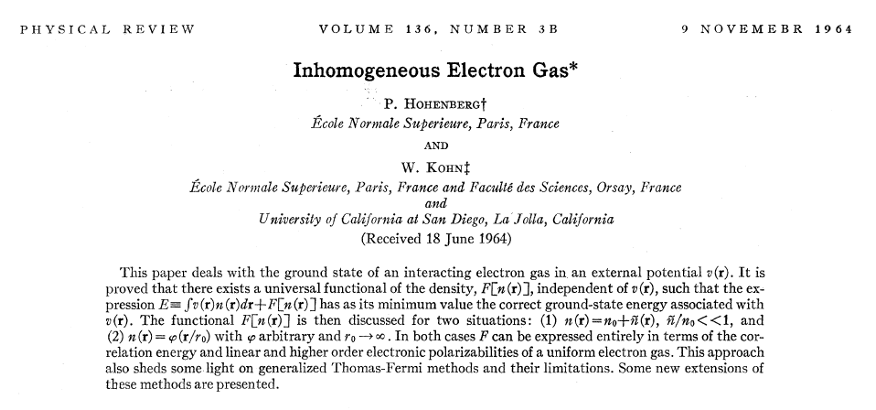
\includegraphics[width=\linewidth]{lectures/figures/5_DFT_paper1.png}
            \end{subfigure}
            \begin{subfigure}{0.45\textwidth}
                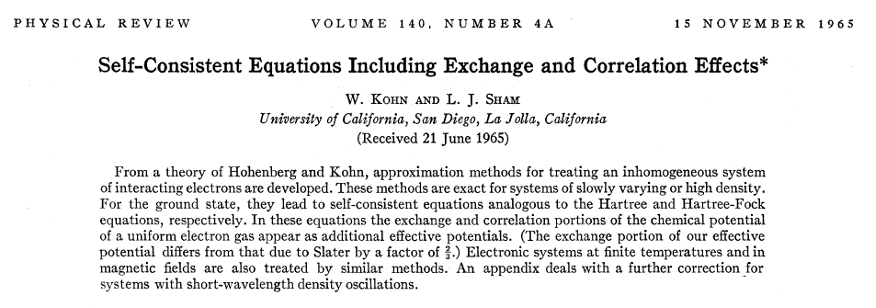
\includegraphics[width=\linewidth]{lectures/figures/5_DFT_paper2.png}
            \end{subfigure}
        \end{figure}
        Collectively more than 100,000 citations as of 2024!
    \end{frame}

    \begin{frame}{Other DFT papers in the top 10 cited papers of all time}
        \begin{columns}
            \column{0.3\textwidth}
            \begin{figure}
                \centering
                
\includegraphics[width=\linewidth]{lectures/figures/5_paper_mountain.jpg}
                \caption{From ref \cite{vannoordenTop100Papers2014}}
            \end{figure}
            \column{0.7\textwidth}
            \# 7: Lee, C. T.; Yang, W. T.; Parr, R. G. Development Of The Colle-Salvetti Correlation-Energy Formula into A Functional Of The Electron-Density. Physical Review B 1988, 37, 785–789.\cite{leeDevelopmentColleSalvettiCorrelationEnergy1988}\newline
            \newline
            \# 8: Becke, A. D. Density‐functional Thermochemistry. III. The Role of Exact Exchange. The Journal of Chemical Physics 1993, 98 (7), 5648–5652. https://doi.org/10.1063/1.464913.\cite{beckeDensityFunctionalThermochemistry1993}

        \end{columns}
    \end{frame}

    \begin{frame}{The Hohenberg-Kohn Theorems}
        \begin{alertblock}{Hohenberg-Kohn Existence Theorem}
            For any system of interacting particles in an external potential $V_{ext}(\vec{r})$, the density is uniquely determined (in other words, the external potential is a unique functional of the density).
        \end{alertblock}

        \begin{alertblock}{Hohenberg-Kohn Variational Theorem}
            A universal functional for the energy $E[n]$ can be defined in terms of the density. The exact ground state is the global minimum value of this functional.
        \end{alertblock}

    \end{frame}

    \begin{frame}{Proof of H-K Existence Theorem}

        \begin{columns}
            \column{0.6\textwidth}
            Assume there are two different external potentials, $V_a$ and $V_b$ with corresponding Hamiltonians $H_a$ and $H_b$ that lead to the same ground state density, $\rho_0$. The ground state wave function and energy are $\psi_0$ and $E_0$, respectively.

            From the variational theorem,

            \begin{eqnarray*}
                E_{0,a} & < & \bra{\psi_{0,b}}H_a\ket{\psi_{0,b}}\\
                E_{0,a} & < & \bra{\psi_{0,b}}(H_a-H_b)\ket{\psi_{0,b}} +  \bra{\psi_{0,b}}H_b\ket{\psi_{0,b}}\\
                E_{0,a} & < & \bra{\psi_{0,b}}(V_a-V_b)\ket{\psi_{0,b}} + E_{0,b}\\
                E_{0,a} & < & \int (V_a-V_b)\rho_0(\vec{r})  d \vec{r} + E_{0,b}\\
            \end{eqnarray*}
            \column{0.4\textwidth}
            Using the same argument by swapping $a$ and $b$,

            \begin{eqnarray*}
                E_{0,b} & < & \int (V_b-V_a)\rho_0(\vec{r})  d \vec{r} + E_{0,a}\\
            \end{eqnarray*}

            Summing the two equations, we have

            \begin{eqnarray*}
                E_{0,a} + E_{0,b} & < & E_{0,b} + E_{0,a}
            \end{eqnarray*}

            This is a contradiction, i.e., the original assumption that $V_a$ and $V_b$ lead to the same $\rho_0$ must be false.

        \end{columns}

    \end{frame}



    \begin{frame}{Consequence of H-K theorems}
        Schr\"odinger equation in 3N electronic coordinates reduced to solving for electron density in 3 spatial coordinates!\newline
        \newline
        In theory, H-K theorems are exact.\newline
        \newline
        Unfortunately, no recipe for what the functional is.\newline
        \newline
        In other words, beautiful theory, but practically useless (until one year later…)

    \end{frame}


    \begin{frame}{A change of notation}
        Electronic Hamiltonian (atomic units)
        \begin{eqnarray*}
            H & = & -\sum_i \frac{1}{2}\nabla_i^2
            -\sum_i\sum_k \frac{Z_k}{r_{ik}}
            +\sum_i\sum_j \frac{1}{r_{ij}}\\
            & = & T + V_{ne} + V_{ee}
        \end{eqnarray*}

        From H-K theorem, energy (and everything) is a functional of the density. Therefore,

        \begin{equation*}
            E[\rho(\vec{r})] = T[\rho(\vec{r})] + V_{ne}[\rho(\vec{r})] + V_{ee}[\rho(\vec{r})]
        \end{equation*}

    \end{frame}


    \begin{frame}{Kohn-Sham Ansatz}
        Fictitious system of electrons that do not interact and live in an external potential (Kohn-Sham potential) such that ground-state charge density is identical to charge density of interacting system.\cite{shamDensityFunctionalTheoryEnergy1983} We can then break down the energy into non-interacting electron contributions and add corrections for the interactions:
        \begin{equation*}
            E[\rho(\vec{r})] = T_{ni}[\rho(\vec{r})] + V_{ne}[\rho(\vec{r})] + V_{ee}[\rho(\vec{r})] + \Delta T[\rho(\vec{r})] + \Delta V_{ee} [\rho(\vec{r})]
        \end{equation*}

        The contribution from the correction terms ($\Delta T[\rho(\vec{r})]$ and $\Delta V_{ee} [\rho(\vec{r})]$) is called the \textbf{exchange-correlation energy}.

    \end{frame}

    \begin{frame}{Kohn-Sham Equations}

        \begin{eqnarray*}
            E[\rho(\vec{r})] & = & \sum_i [ -\frac{1}{2} \int \psi_i^*(\vec{r}) \nabla^2 \psi_i(\vec{r}) d\vec{r}
            - \sum_k \int \psi_i^*(\vec{r})\frac{Z_k}{r_{ik}} \psi_i(\vec{r}) d\vec{r}  \\
            & + &  \frac{1}{2} \int \int \frac{\rho(\vec{r'})}{|\vec{r}-\vec{r'}|}|\psi_i(\vec{r})|^2 d\vec{r}d\vec{r'} ]+ E_{xc}[\rho(\vec{r})]\\
            h_i^{KS} & = & -\frac{1}{2} \nabla^2
            - \sum_k \frac{Z_k}{r_{ik}} + \frac{1}{2} \frac{\rho(\vec{r'})}{|\vec{r}-\vec{r'}|}+ V_{xc}[\rho(\vec{r})]
        \end{eqnarray*}

        where
        \begin{eqnarray*}
            h_i^{KS} \psi_i(\vec{r}) & = & \varepsilon_i \psi_i(\vec{r}) \\
            \rho(\vec{r}) &=& |\psi_i(\vec{r})|^2
        \end{eqnarray*}
    \end{frame}

    \begin{frame}{Solution to KS equations}
        Follows broadly the same procedure as the HF SCF approach, i.e., construct guess KS orbitals within a basis set, solve secular equation to obtain new orbitals (and density matrix) and iterate until convergence.\newline
        \newline
        Key differences between HF and DFT
        \begin{itemize}
            \item HF is approximate, but can be solved exactly.
            \item DFT is formally exact, but solutions require approximations ($V_{xc}$).
        \end{itemize}

    \end{frame}

    \begin{frame}{Flowchart for KS solution}
        \begin{figure}
            \centering
            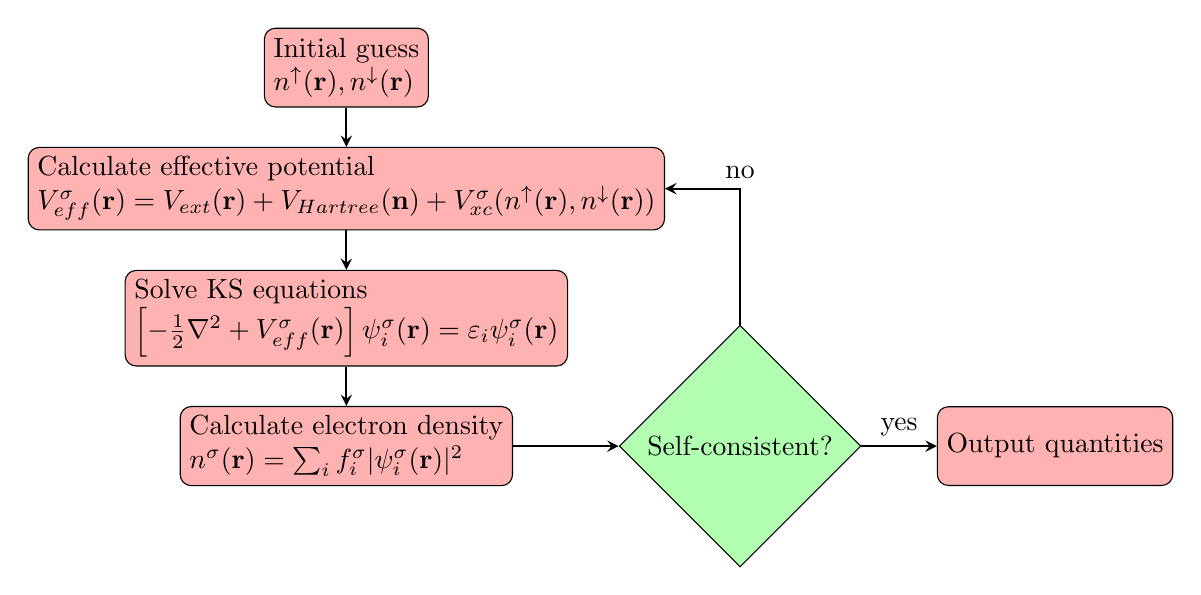
\begin{tikzpicture}[node distance=0.5cm]
                \tikzstyle{roundrect} = [rectangle, rounded corners, minimum width=2cm, minimum height=1cm, draw=black, fill=red!30]
                \tikzstyle{decision} = [diamond, minimum width=3cm, minimum height=1cm, text centered, draw=black, fill=green!30]

                \tikzstyle{arrow} = [thick,->,>=stealth]
                \node (initial) [roundrect, align=left] {Initial guess \\$n^\uparrow(\vec{r}),n^\downarrow(\vec{r})$};
                \node (effectivepot) [roundrect, below=of initial, align=left] {Calculate effective potential\\$V_{eff}^\sigma(\vec{r})=V_{ext}(\vec{r}) + V_{Hartree}(\vec{n}) + V_{xc}^\sigma(n^\uparrow(\vec{r}),n^\downarrow(\vec{r}))$};
                \node (solveks) [roundrect, below=of effectivepot, align=left] {Solve KS equations\\$\left[ -\frac{1}{2} \nabla^2 + V_{eff}^\sigma(\vec{r}) \right] \psi_i^\sigma(\vec{r}) = \varepsilon_i \psi_i^\sigma(\vec{r}) $};
                \node (electrondens) [roundrect, below=of solveks,align=left] {Calculate electron density\\$n^\sigma(\vec{r}) = \sum_i f_i^\sigma|\psi_i^\sigma(\vec{r})|^2$};
                \node (converge) [decision, right of =electrondens, node distance=5cm] {Self-consistent?};
                \node (output) [roundrect, right of =converge, node distance=4cm] {Output quantities};

                \draw [arrow] (initial) -- (effectivepot);
                \draw [arrow] (effectivepot) -- (solveks);
                \draw [arrow] (solveks) -- (electrondens);
                \draw [arrow] (electrondens) -- (converge);
                \draw [arrow] (converge) -- node[anchor=south] {yes} (output);
                \draw [arrow] (converge) |- node[anchor=south] {no} (effectivepot);
            \end{tikzpicture}
        \end{figure}
    \end{frame}

    \begin{frame}{Exchange-correlation functional}

        \begin{equation*}
            E[\rho(\vec{r})] = T_{ni}[\rho(\vec{r})] + V_{ne}[\rho(\vec{r})] + V_{ee}[\rho(\vec{r})] + V_{xc}[\rho(\vec{r})]
        \end{equation*}

        Thus far, we have constructed an elegant system, but we have conveniently swept all unknowns into the mysterious $V_{xc}$. \newline
\newline 
Unfortunately, the H-K theorems provide no guidance on the form of this $V_{xc}$. With approximate$V_{xc}$, DFT can be non-variational.\newline
        \newline
        What is the simplest possible assumption we can make?
    \end{frame}

    \begin{frame}{Local Density Approximation (LDA)}

        \begin{columns}
            \column{0.3\textwidth}
            \begin{figure}
                \centering
                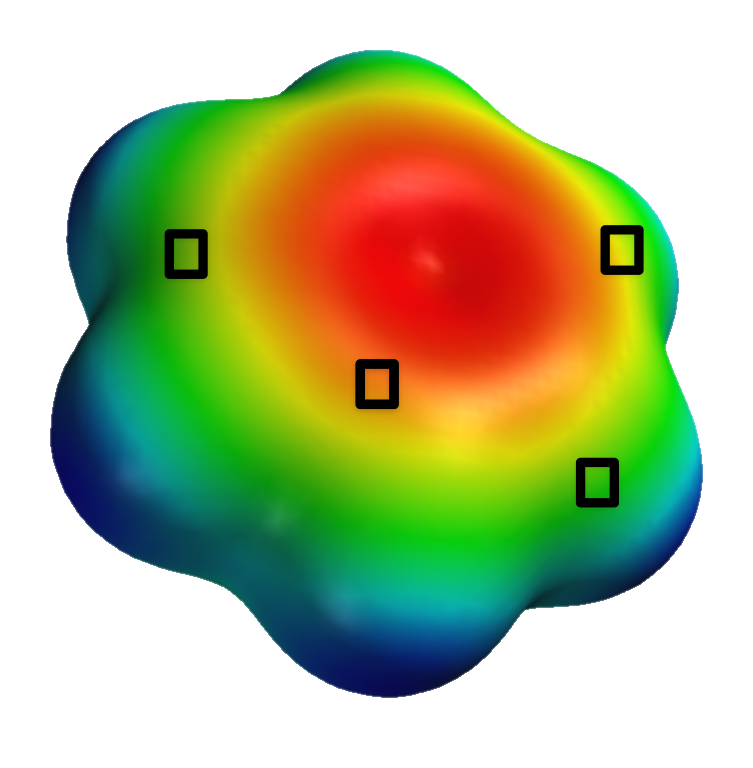
\includegraphics[width=0.8\linewidth]{lectures/figures/5_LDA.png}
            \end{figure}
            \column{0.7\textwidth}
            Approximate $V_{xc}$ as a local or nearly local functional of density.\newline
            \newline
            Total XC energy is given by integrating the local XC energy of a homogenous electron gas with the same density at each coordinate.

            \begin{equation*}
                E_{xc}^{LDA}[\rho^\uparrow, \rho^\downarrow] = \int \rho(\vec{r})[\varepsilon_x^{hom}(\rho^\uparrow, \rho^\downarrow)+\varepsilon_c^{hom}(\rho^\uparrow, \rho^\downarrow)] d\vec{r}
            \end{equation*}

        \end{columns}

    \end{frame}

    \begin{frame}{Exchange-Correlation for a Homogenous Electron Gas}

        Exchange energy can be analytically derived as:
        \begin{equation*}
            E_x^\sigma[\rho] = -\frac{3}{4}\left( \frac{6}{\pi} \rho^\sigma \right)^{1/3}
        \end{equation*}

        Correlation energy for HEG has been accurately calculated using quantum Monte Carlo methods.\cite{ceperleyGroundStateElectron1980}
        \begin{figure}
            \centering
            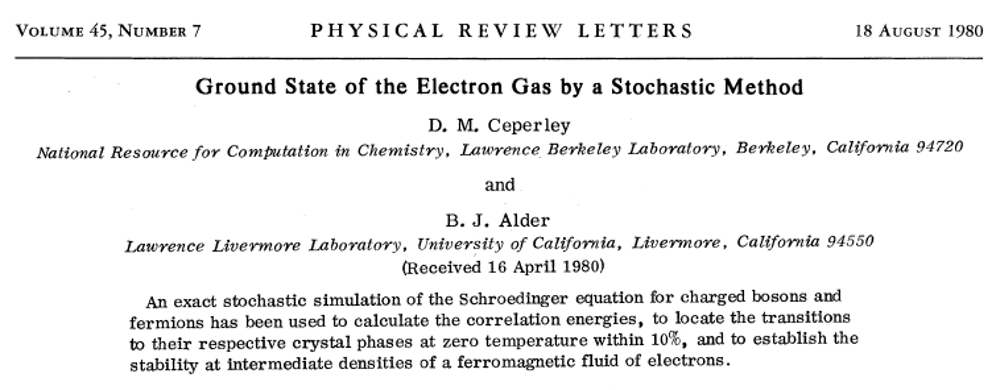
\includegraphics[width=0.7\linewidth]{lectures/figures/5_LDA_Corre.png}
        \end{figure}
    \end{frame}

    \begin{frame}{Does LDA work?}

        \begin{figure}
            \centering
            \begin{subfigure}{0.6\textwidth}
                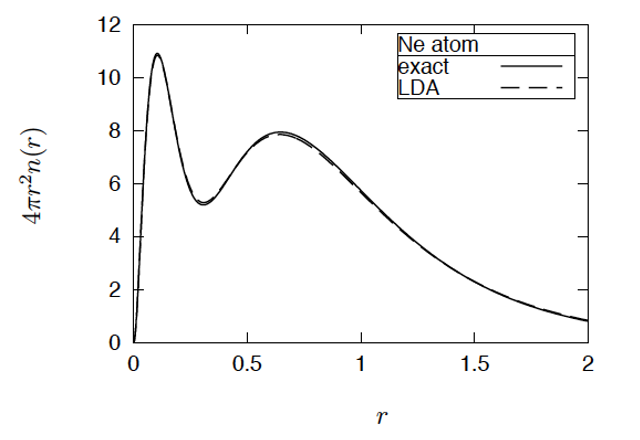
\includegraphics[width=\linewidth]{lectures/figures/5_radial_density_Ne.png}
                \caption{Electron density agreement is good.}
            \end{subfigure}
            \begin{subfigure}{0.35\textwidth}
                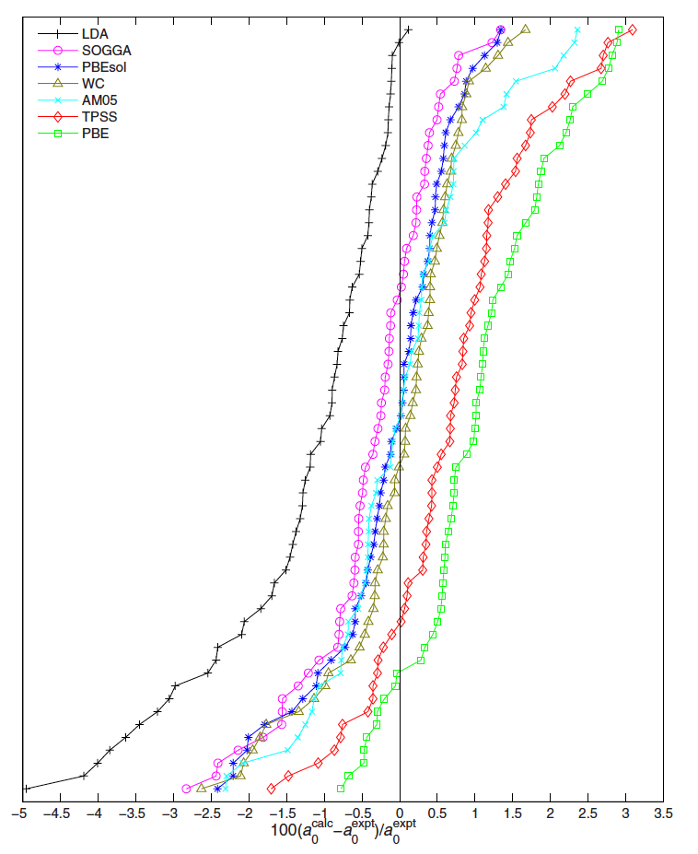
\includegraphics[width=\linewidth]{lectures/figures/5_bond_lengths.png}
                \caption{Overbinding is evident for LDA.\cite{haasCalculationLatticeConstant2009}}
            \end{subfigure}
        \end{figure}

    \end{frame}

    \begin{frame}{Error in LDA xc energy density of Si}
        Exchange energies are too low and correlation energies that are too high $\implies$ Cancellation of errors!
        \begin{figure}
            \centering
            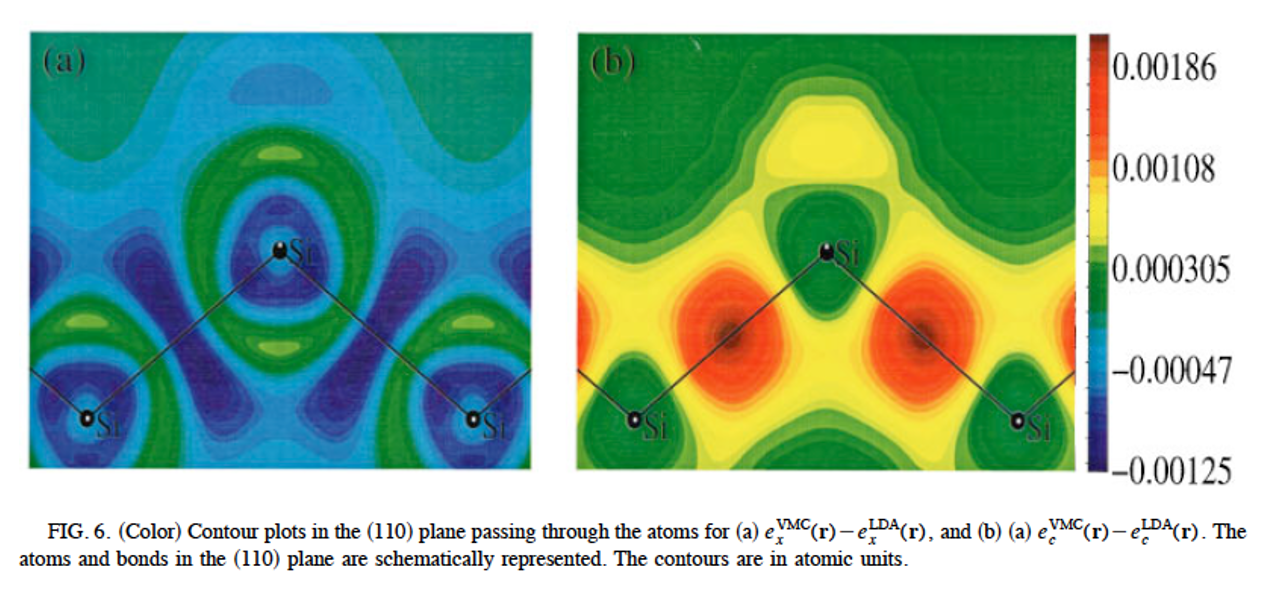
\includegraphics[width=0.7\linewidth]{lectures/figures/5_xc_energies_Si.png}
            \caption{From \cite{hoodExchangeCorrelationSilicon1998}}
        \end{figure}

    \end{frame}

    \begin{frame}{Phases of Si from LDA – an early success story}
        \begin{figure}
            \centering
            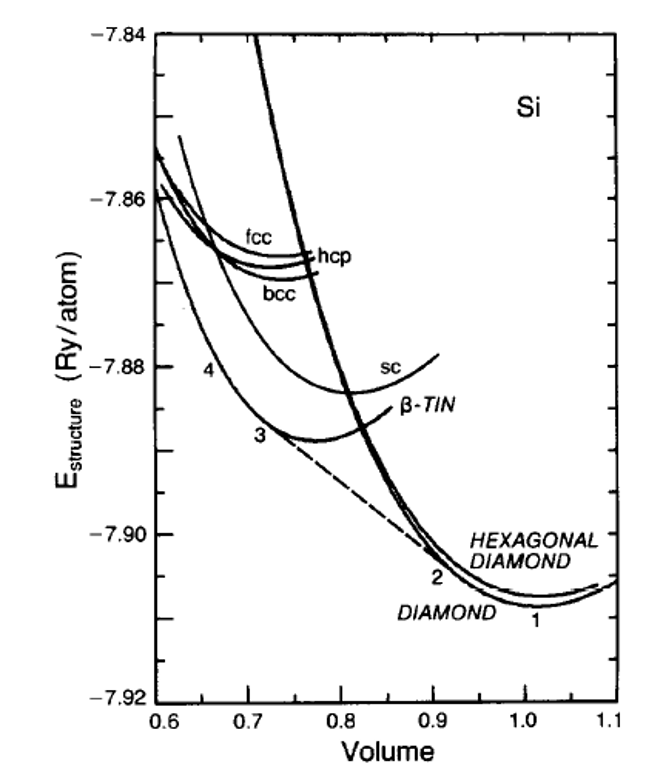
\includegraphics[width=0.35\linewidth]{lectures/figures/5_phase_diagram_si.png}
            \caption{From \cite{yinTheoryStaticStructural1982}.}
            \label{fig:enter-label}
        \end{figure}
    \end{frame}

    \begin{frame}[allowframebreaks]{Bibliography}
        \bibliographystyle{unsrt}
        \bibliography{refs}
    \end{frame}

    \begin{frame}
        \Huge{\centerline{The End}}
    \end{frame}

\end{document}

